\documentclass[12pt]{article}
\usepackage{graphicx}
\usepackage[margin=0.8in]{geometry}
\begin{document}
{\bf Names:} Jack Bracewell, Milan Misak, Craig Ellis \\
{\bf Usernames:} jb2910, mm5510, ce710 \\
{\bf Group Number: 28}  \\ \\

\section*{Assignment 5: T-test}

\subsubsection*{Which algorithm performed better overall in terms of values of $F_1$ measure (part I)? Which algorithm performed better when comparison was performed using the t-test (part II and part III)? Can we claim that this algorithm is a better learning algorithm than the others in general? Why? Why not?}

The neural networks algorithm performed best in terms of values of $F_1$ measure.

\subsubsection*{How did you adjust the significance level in order to take into account the fact that you perform a multiple comparison test?}

divide $\alpha$ by k.

\subsubsection*{Which type of t-test did you use and why?}

The special kind.

\subsubsection*{Why do you think t-test was performed on the classification error and not the F1 measure?}

Something about classification error having higher varience maybe.

\subsubsection*{What is the trade-off between the number of folds you use and the number of examples per fold? In other words, what is going to happen if you use more folds, so you will have fewer examples per fold, or if you use fewer folds, so you will have more examples per fold?}

This shan't be too difficult.

\subsubsection*{Suppose that we want to add some new emotions to the existing dataset. Which of the examined algorithms are more suitable for incorporating the new classes in terms of engineering effort? Which algorithms need to undergo radical changes in order to include new classes?}

Surely CBR is the easiest? Neural networks will need new optimal shit so that might be hardest?

\subsection*{Implementation details}
\begin{itemize}
  \item RETRIEVE:
    We Cycle through all the cases in the structure, picking the cases with the 3 highest similarities to the case we are attempting to classify (3-NN). If there are more than 3 with the highest similarity then they are all included in the "voting", and not discarded. For example, case one has a similarity of 79, case two has 78, and cases three and four both have similarities of 77. We cannot decide which of cases three and four to keep in the 'top three', so we include both.
  \item REUSE:
    We simply assign the solution value from the retrieved case to the case we are classifying.
  \item RETAIN:
    A new case is made with the corresponding AU Vector and solution that was found. The weight is a value used for calculating similarity, and is set to 0.8 for every new case, because that is roughly the classification rate, ie - how much we should trust the prediction, compared to the training data which we know is correct.
  \item CBR cases:
    Each case has an AUVector, a solution, and a typicality value, the use of which is explained previously.
\end{itemize}

\subsection*{Evaluation results}

\begin{table}
\centering
\begin{tabular}{r r | r r r r r r}
\multicolumn{8}{c}{Predicted class} \\
&  & Anger & Disgust & Fear & Happiness & Sadness & Surprise \\
\hline
 & Anger            & 9.6 & 1.3  & 0.6 & 0.9  & 0.5 & 0.3  \\
 & Disgust          & 1.7 & 14.9 & 0.3 & 1.7  & 0.8 & 0.4  \\
Actual class & Fear & 1.0 & 0.1  & 8.2 & 0.4  & 0.1 & 2.1  \\
 & Happiness        & 0.1 & 0.8  & 0.2 & 19.9 & 0.1 & 0.5  \\
 & Sadness          & 2.4 & 1.8  & 0.9 & 0.9  & 6.6 & 0.6  \\
 & Surprise         & 0.1 & 0.3  & 0.7 & 0.4  & 0.1 & 19.1 \\
\end{tabular} 
\caption{Confusion matrix}
\end{table}

\begin{table}
\centering
\begin{tabular}{l | r r}
Emotion & Recall rate (\%) & Precision rate (\%) \\
\hline
Anger     & 72.7273 & 64.4295 \\
Disgust   & 75.2525 & 77.6042 \\
Fear      & 68.9076 & 75.2294 \\
Happiness & 92.1296 & 82.2314 \\
Sadness   & 50.0000 & 80.4878 \\
Surprise  & 92.2705 & 83.0435 \\
\end{tabular}
\caption{Recall and precision rates}
\end{table}

\begin{table}
\centering
\begin{tabular}{l | r}
Emotion & \( F_1 \) measure \\
\hline
Anger     & 68.3274 \\
Disgust   & 76.4103 \\
Fear      & 71.9298 \\
Happiness & 86.8996 \\
Sadness   & 61.6822 \\
Surprise  & 87.4142 \\
\end{tabular}
\caption{F1 measures}
\end{table}

Average classification rate = 0.7830 \\ \\

Confusion matrix: the confusion matrix shows that our cbr performs fairly well. Sadness, however, is often misclassified as other classes, specifically Anger. Anger itself is chosen fairly often to classify any case (meaning many emotions are often mistaken for anger). \\
Classification rate: Not as good as some previous classification methods (eg. neural networks), it is still always over 70\%, and almost always above 75\%, after some tweaking of the k nearest neighbours and the weight given to classified cases, which is a reasonable success rate. \\
Recall/Precision rate: These are fairly high for most emotions, with just a few cases bringing the average right down. Sadness, for example, was only recognised correctly 50\% of the time, and fear only 68\%. As stated before, anger was often used incorrectly as a classification, resulting in its low precision rate. The $F_1$ measure confirms this, with all emotions but sandness and anger scoring above 70\%. \\

\newpage
\subsection*{Code Flowchart}

TODO
%\begin{center}
%  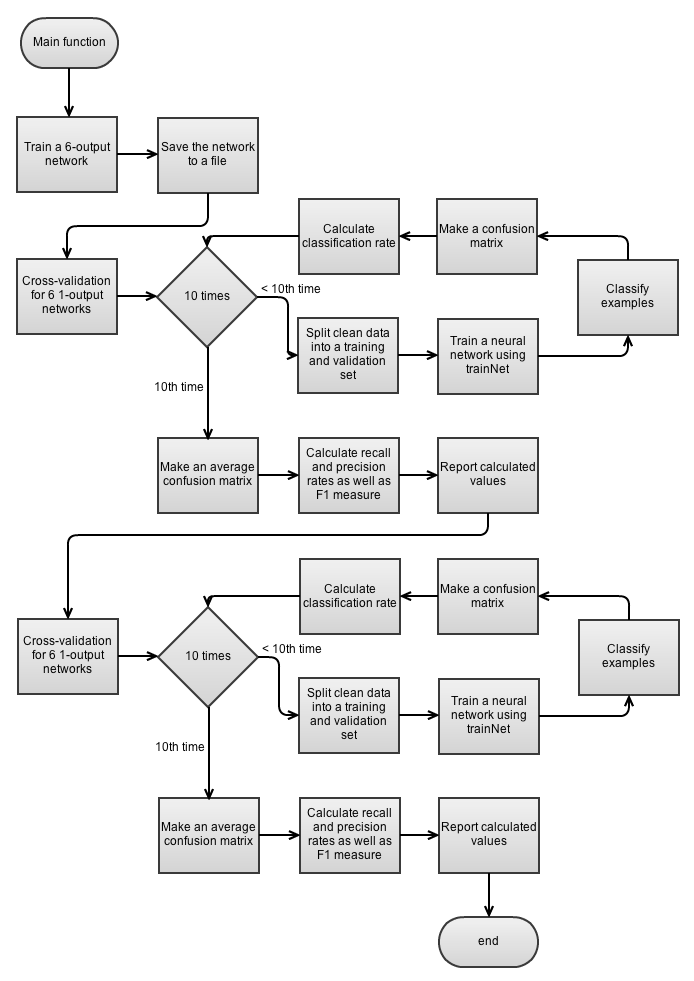
\includegraphics[scale=0.7]{report-images/main.png}
%\end{center}



\end{document}
